\documentclass[10pt, xcolor=x11names,compress]{beamer}
\usepackage{tabulary}
\usepackage{booktabs}
\usepackage{float}
\usepackage{graphicx}
\usepackage{mwe}% for example pictures
\usepackage{siunitx}
\usepackage{hyperref}

\usecolortheme{spruce}
\useoutertheme{infolines}
\usefonttheme[onlymath]{serif}
\setbeamertemplate{headline}[default]
\setbeamertemplate{navigation symbols}{}
\mode<beamer>{\setbeamertemplate{blocks}[rounded][shadow=true]}
\setbeamercovered{transparent}
\setbeamercolor{block body}{use=structure, fg=white, bg=black!20}
\setbeamercolor{itemize item}{fg=black}
\setbeamercolor{itemize subitem}{fg=gray} 
\setbeamercolor{itemize subsubitem}{fg=black!20} 
\makeatletter\setbeamertemplate{footline}
{  
\leavevmode%  
\hbox{%  
\begin{beamercolorbox}[wd=.5\paperwidth,ht=2.5ex,dp=1ex,center]{author in head/foot}%    
\usebeamerfont{author in head/foot}
\insertshortauthor%~~\beamer@ifempty{\insertshortinstitute}{}
 \end{beamercolorbox}%  
 
 % \begin{beamercolorbox}[wd=.333333\paperwidth,ht=2.5ex,dp=1ex,center]{institute in head/foot}%    
 % \usebeamerfont{title in head/foot}\insertinstitute  
 % \end{beamercolorbox}%  
 
 \begin{beamercolorbox}[wd=.5\paperwidth,ht=2.5ex,dp=1ex,right]{date in head/foot}%    
 \usebeamerfont{date in head/foot}\insertshortdate{}\hspace*{2em}    
 \insertframenumber{} / \inserttotalframenumber\hspace*{2ex}   
 \end{beamercolorbox}}%  
 \vskip0pt%
 }
 \makeatother 
 \useoutertheme[footline=empty, subsection=false]{miniframes}
 \usepackage{multicol}  
 \author{Chaoqi Wang, Ziyu Ye}
 \author[C. Wang, Z. Ye, Z. Feng, A. Badanidiyuru, H. Xu]{Chaoqi Wang\inst{1}, Ziyu Ye\inst{1}, Zhe Feng\inst{2}\\Ashwinkumar Badanidiyuru\inst{2}, Haifeng Xu\inst{1}}

\institute[The University of Chicago]{The University of Chicago\inst{1}\\Google Research\inst{2}}
 \title{Follow-ups Also Matter:\\Improving Contextual Bandits via Post-serving Contexts}

 \date{NeurIPS 2023} 
 \begin{document}
 \begin{frame}
 \titlepage
 \end{frame}

\section{Introduction}
\begin{frame}[label=Background]{Background}
\begin{itemize}
\item Here to input your background\\
   \begin{itemize}
    \item This is the sub-content
    \item Here you can also jump to other slides \hyperlink{Rocky}{\beamergotobutton{go}}
   \end{itemize}
\item Now we go back to the main content\\

\end{itemize}
\end{frame}

\section{Literature Review}
\begin{frame}{Here is the title of this slides}
\begin{itemize}
    \item Studies investigating the impact of Rocky's little brother's birth on his instances of running away. 
    \begin{figure}
        \centering
        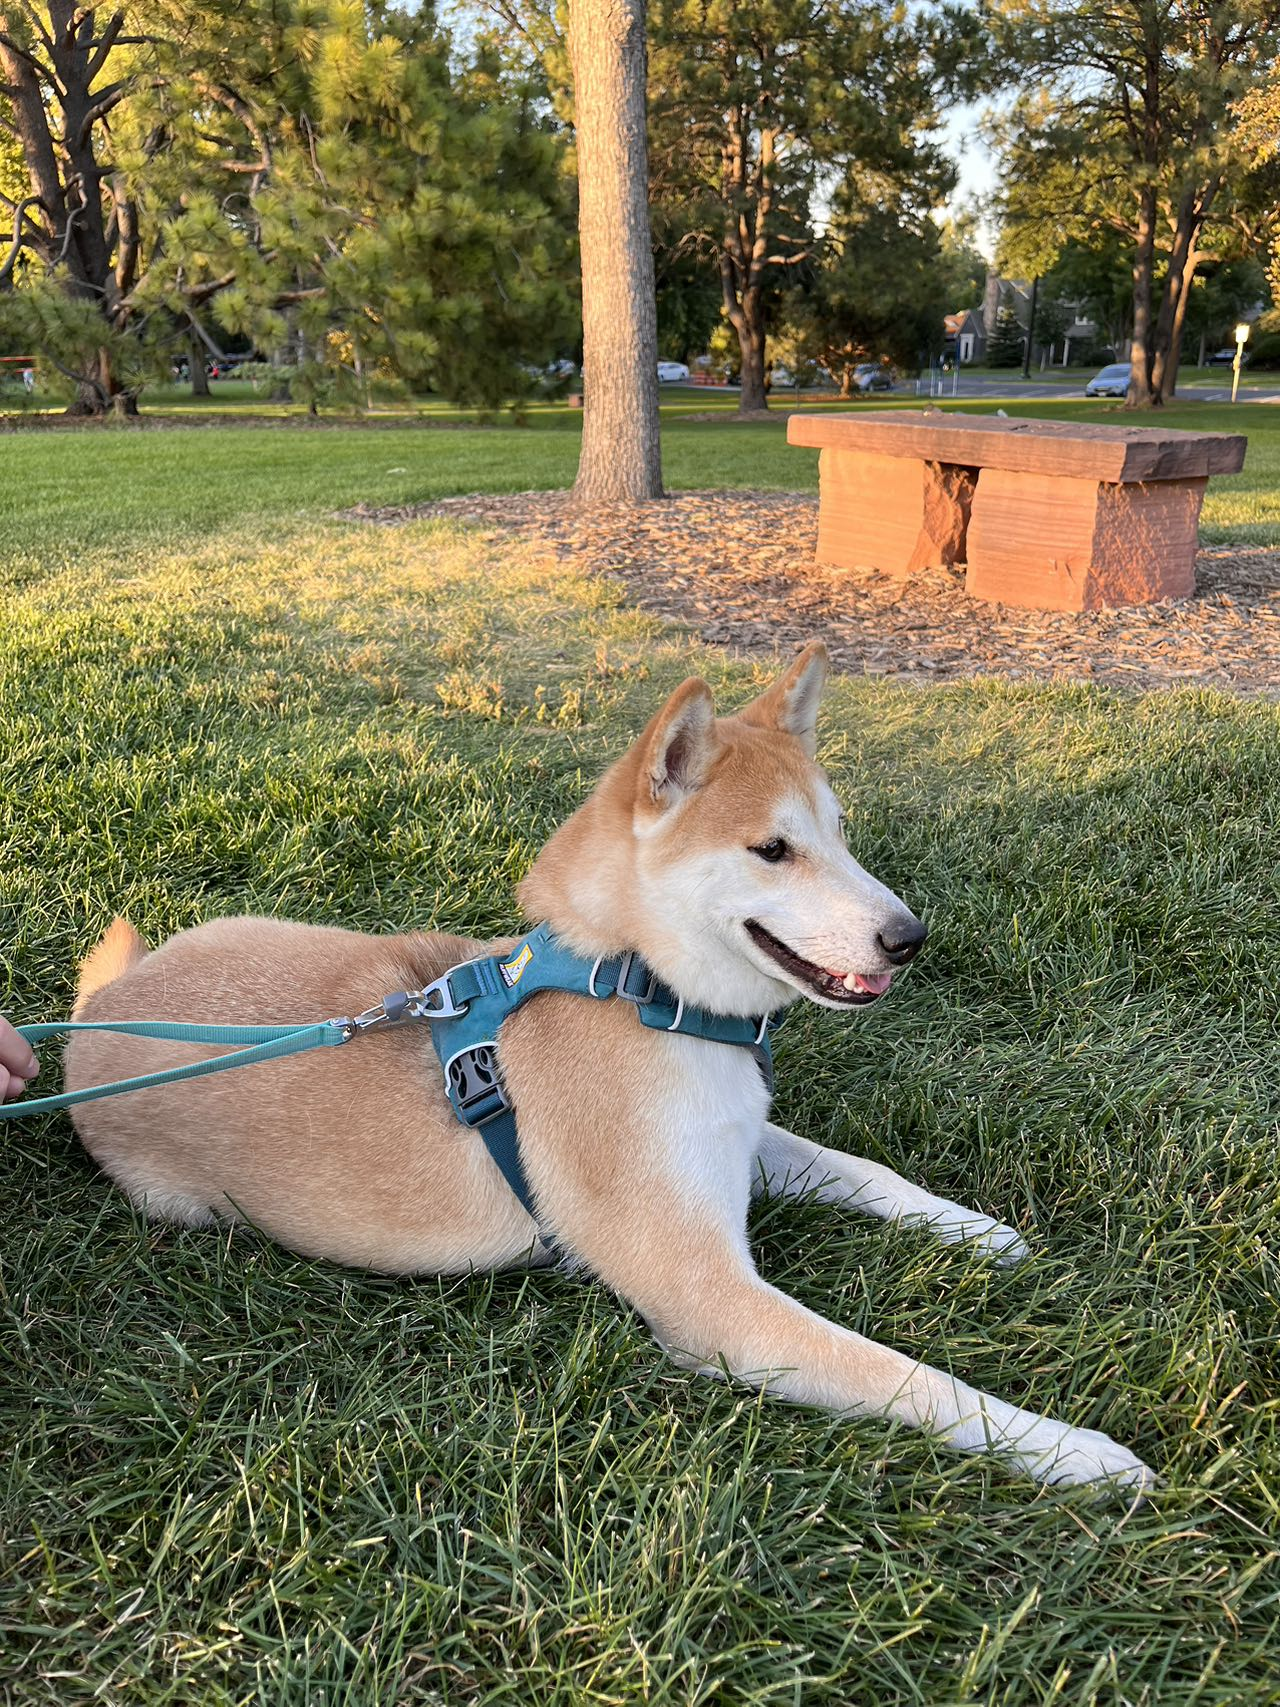
\includegraphics[width=0.3\textwidth]{Figure1.jpg}
        \caption{His name is Rocky}
        \label{fig:enter-label}
    \end{figure}
\end{itemize}
\end{frame}

\section{Method}
\begin{frame}[label=Rocky]{There you can also separate the page}
\begin{figure}
 \begin{columns}[c]
  \begin{column}{0.3\textwidth}
    \centering
    
\includegraphics[width=1\textwidth]{Figure2.jpg}
  \end{column}
  \begin{column}{0.3\textwidth}
    \centering
    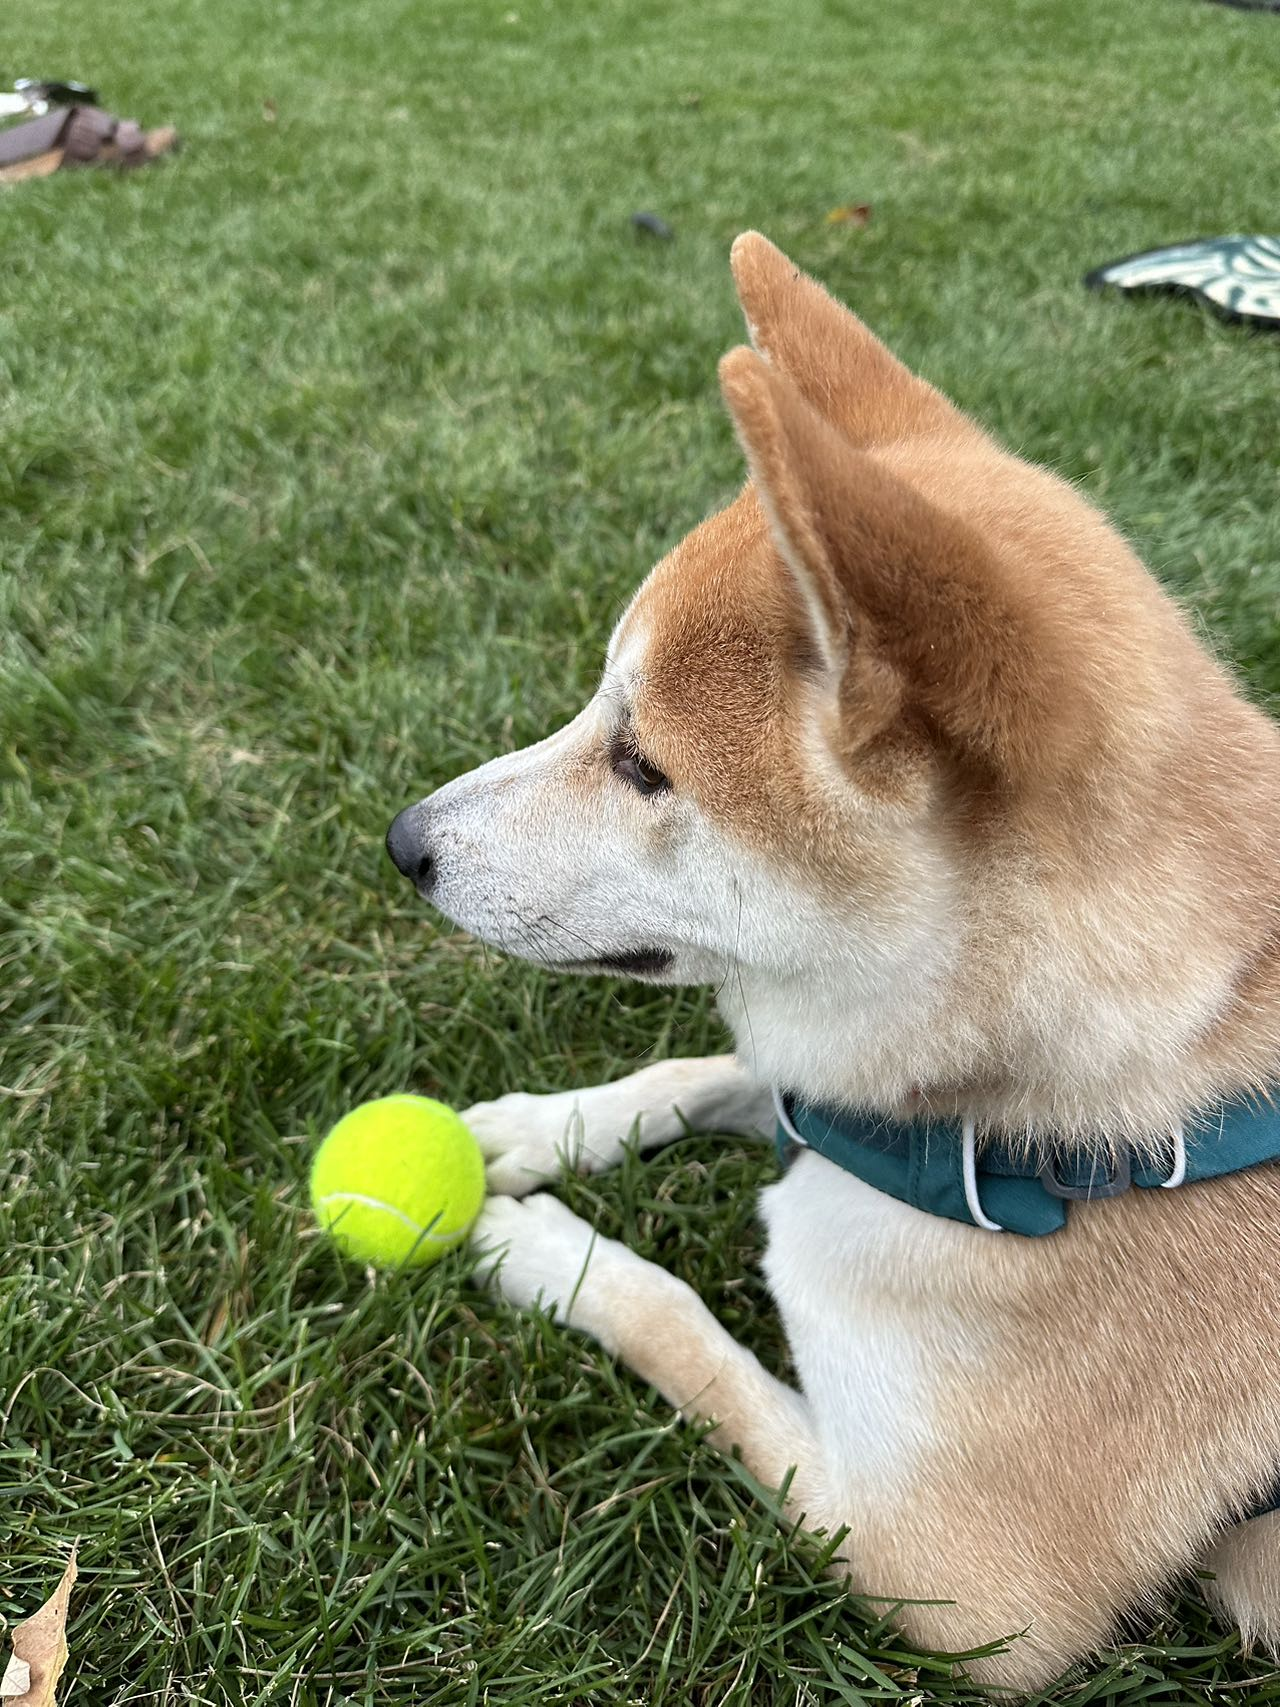
\includegraphics[width=1\textwidth]{Figure3.jpg}
  \end{column}
  \end{columns}
  \caption{Here I just using one caption for these 2 cute pictures but you can also using 2 captions  \parbox{\linewidth}{\small\textit{Data source: Rocky's daily look}}}
\end{figure}
Now I am going back to the previous slidesby clicking this: \hyperlink{Background}{go back}
\end{frame}
 



\begin{frame}
 \begin{center}
		{\Huge Thank you!}\\
		\bigskip\bigskip % Vertical whitespace
		
	\end{center}
\end{frame}

\end{document}